\documentclass[9.5pt,a4paper]{article}
\usepackage[margin=1.2cm,headheight=1.2cm,headsep=6pt,footskip=14pt]{geometry}
\usepackage{graphicx}
\usepackage{fancyhdr}
\usepackage{booktabs}
\usepackage{tabularx}
\usepackage{array}
\usepackage{amsmath,amssymb}
\usepackage{microtype}
\usepackage{hyperref}

\hypersetup{
    colorlinks=true,
    linkcolor=black,
    urlcolor=black,
    citecolor=black
}

% Header / Footer
\pagestyle{fancy}
\fancyhf{}
\fancyhead[L]{%
  \begin{tabular}{@{}c@{\hspace{5pt}}l@{}}
    
\includegraphics[width=0.9cm]{fast_logo.png} & \textbf{FAST NUCES, Islamabad Campus}\\
    & {\scriptsize Department of Computer Science, Fall 2026}
  \end{tabular}%
}
\fancyhead[R]{%
  \begin{tabular}{@{}r@{}}
    \textbf{CS2001: Data Structures}\\
    \textbf{Assignment 2: ImageLab (Phase 1)}\\
    Ahmad Ali \textbar{} 25-i0817 \textbar{} Section E
  \end{tabular}%
}
\fancyfoot[L]{\scriptsize FAST NUCES Islamabad}
\fancyfoot[C]{\scriptsize CS2001 Data Structures}
\fancyfoot[R]{\scriptsize Page \thepage\ of 3}
\renewcommand{\headrulewidth}{0.4pt}
\renewcommand{\footrulewidth}{0.4pt}

\begin{document}

% =========================================================================
% PAGE 1: COVER AND OVERVIEW
% =========================================================================
\thispagestyle{empty}
\vspace*{1.0cm}

\begin{center}
    
\includegraphics[width=3.0cm]{fast_logo.png}\\[12pt]
    {\LARGE \textbf{National University of Computer and Emerging Sciences}}\\[4pt]
    {\large \textbf{Islamabad Campus \textbar{} Department of Computer Science}}\\[12pt]
    \rule{0.88\textwidth}{0.8pt}\\[10pt]
    {\huge \textbf{CS2001: Data Structures}}\\[6pt]
    {\Large \textbf{Assignment 2: ImageLab (Phase 1 Technical Report)}}\\[10pt]
    \rule{0.88\textwidth}{0.8pt}\\[20pt]

    \vspace{0.4cm}
    \begin{tabular}{|p{0.78\textwidth}|}
        \hline
        \centering
        \vspace{4pt}
        {\Large \textbf{Student Information}}\\[6pt]
        \begin{tabular}{ll}
            \textbf{Student Name:} & Ahmad Ali \\[4pt]
            \textbf{Roll Number:}  & 25-i0817 \\[4pt]
            \textbf{Section:}      & BS CS E \\[4pt]
            \textbf{Course:}       & CS2001 Data Structures \\[4pt]
            \textbf{Deliverable:}  & Phase 1 Final Submission (16/10/2026) \\[4pt]
        \end{tabular}
        \vspace{4pt}
        \tabularnewline
        \hline
    \end{tabular}
\end{center}

\vspace{0.6cm}
\section*{Phase 1 Project Summary and Rubric Overview}
This report explains the implementation of Phase 1 of ImageLab. Every component is written from scratch without forbidden library containers or templates. All requirements match the marks distribution in Section 8 of the assignment rubric:

\begin{itemize}
    \item \textbf{Section 6.1 (8 Marks):} Hand written core image operations on raw pixel grids.
    \item \textbf{Section 6.2 (7 Marks):} Custom dynamic array stack implementation.
    \item \textbf{Section 6.3 (9 Marks):} Undo and redo engine using two stacks.
    \item \textbf{Section 6.4 (7 Marks):} Custom circular queue implementation.
    \item \textbf{Section 6.5 (6 Marks):} Job processing pipeline with bounded capacity.
    \item \textbf{Section 6.6 (8 Marks):} Stack based and queue based bucket fill algorithms.
    \item \textbf{Section 6.7 and 6.8 (5 Marks):} Data structure inspector and full test coverage.
\end{itemize}

\section{Section 6.1: Core Image Operations Implemented by Hand (8 Marks)}
\begin{itemize}
    \item \textbf{Raw Pixel Grid:} Images are stored as a 2D dynamic array of pixels using \texttt{Pixel**} allocated on the heap.
    \item \textbf{Crop:} Extracts any valid rectangular subregion from coordinate $(x_1, y_1)$ to $(x_2, y_2)$ into a new grid.
    \item \textbf{Rotation:} Supports clockwise rotation for 90, 180, and 270 degrees. Rotation by 180 degrees is done in place by swapping opposite pixels.
    \item \textbf{Flip:} Horizontal flip swaps opposite columns across each row. Vertical flip swaps row pointers directly in $\mathcal{O}(H)$ time without touching pixels.
    \item \textbf{Brightness:} Adds a positive or negative intensity value to every pixel. Clamps all values between 0 and 255 to prevent overflow.
    \item \textbf{Grayscale:} Converts colors to shades of gray using standard luminance weights: $0.299 \times R + 0.587 \times G + 0.114 \times B$.
    \item \textbf{Bilinear Resize:} Computes four point weighted average interpolation to scale images up or down smoothly.
    \item \textbf{Box Blur:} Applies a $3 \times 3$ averaging box filter across neighbor pixels using a separate scratch grid.
\end{itemize}

\clearpage

% =========================================================================
% PAGE 2: DATA STRUCTURES AND PIPELINE
% =========================================================================

\section{Section 6.2: Stack Implementation stackType (7 Marks)}
\begin{itemize}
    \item \textbf{Array Based Storage:} Implemented as a template class \texttt{stackType<Type>} using dynamic heap memory.
    \item \textbf{Constant Time Operations:} Push, pop, and top run in strict $\mathcal{O}(1)$ time using an integer index \texttt{stackTop}.
    \item \textbf{Automatic Capacity Expansion:} Stack doubles in capacity dynamically if full, ensuring no push fails during operation.
    \item \textbf{Boundary Safety:} Pop and top on an empty stack are safely intercepted with clear error messages without program crashes.
    \item \textbf{Deep Copy Support:} Custom copy constructor and assignment operator create deep copies of all heap memory.
    \item \textbf{Stack Reset:} The function \texttt{initializeStack()} safely resets the stack to empty in $\mathcal{O}(1)$ time.
\end{itemize}

\section{Section 6.3: Undo and Redo with Two Stacks (9 Marks)}
\begin{itemize}
    \item \textbf{Dual Stack Engine:} Uses an \texttt{undoStack} for past states and a \texttt{redoStack} for future states.
    \item \textbf{Independent Deep Copy Snapshots:} Each undo record stores a deep copy of the image grid so modifying the current image never damages saved history.
    \item \textbf{New Edit Invariant:} When the user performs a new edit, the previous state is pushed to \texttt{undoStack} and \texttt{redoStack} is completely emptied.
    \item \textbf{Undo Execution:} Pops the previous state from \texttt{undoStack}, pushes the current state to \texttt{redoStack}, and restores the canvas.
    \item \textbf{Redo Execution:} Pops the forward state from \texttt{redoStack}, pushes the current state to \texttt{undoStack}, and reapplies the edit.
    \item \textbf{Consecutive Stability:} Multiple undos followed by multiple redos restore images bit for bit with zero memory leaks.
\end{itemize}

\section{Section 6.4: Circular Queue Implementation queueType (7 Marks)}
\begin{itemize}
    \item \textbf{Bounded Ring Buffer:} Implemented as a template class \texttt{queueType<Type>} with fixed maximum capacity.
    \item \textbf{Zero Element Shifting:} Front and rear pointers advance using modular arithmetic: $(index + 1) \pmod{capacity}$.
    \item \textbf{Constant Time Guarantees:} \texttt{addQueue()} and \texttt{deleteQueue()} both operate in strict $\mathcal{O}(1)$ time.
    \item \textbf{Capacity Checking:} \texttt{isEmptyQueue()} and \texttt{isFullQueue()} track element count accurately.
    \item \textbf{Safe Memory Management:} Destructor, copy constructor, and assignment operator handle dynamic arrays properly.
\end{itemize}

\section{Section 6.5: Processing Pipeline (6 Marks)}
\begin{itemize}
    \item \textbf{Add Job:} Adds an image edit task to the pipeline queue; safely rejects incoming jobs when the bounded queue is full.
    \item \textbf{List Jobs:} Displays all pending jobs from front to rear with arrival numbers and status indicators.
    \item \textbf{Process Next Job:} Dequeues the front job, applies the edit, and automatically saves an undo snapshot.
    \item \textbf{Process All Jobs:} Loops until the queue is completely drained, executing all queued edits in arrival order.
    \item \textbf{Cancel Job:} Locates a task by job ID and sets a cancellation flag; the task is safely discarded upon dequeue without shifting elements.
    \item \textbf{Clear Queue:} Discards all waiting jobs instantly and resets the queue size counter to zero.
\end{itemize}

\section{Section 6.6: Bucket Fill Stack and Queue Versions (8 Marks)}
\begin{itemize}
    \item \textbf{Stack Based Fill (DFS):} Explores four directional neighbors depth first using an explicit coordinate stack.
    \item \textbf{Queue Based Fill (BFS):} Explores neighbors in level order concentric waves using a circular queue.
    \item \textbf{Identical Output Proof:} Both algorithms produce bit for bit identical filled pixel regions on identical inputs.
    \item \textbf{Same Color Guard:} Immediately exits if the replacement color matches the seed pixel color, avoiding infinite recursion or loops.
\end{itemize}

\begin{center}
    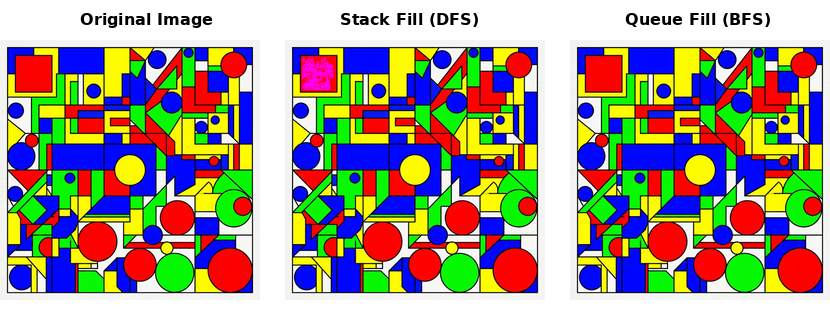
\includegraphics[width=0.82\textwidth,height=3.4cm,keepaspectratio]{bucket_fill_comparison.png}
\end{center}

\clearpage

% =========================================================================
% PAGE 3: COMPLEXITY, INSPECTOR AND TEST EVIDENCE
% =========================================================================

\section{Section 6.7: Data Structure Inspector (Section 6.7 and 6.8)}
\begin{itemize}
    \item \textbf{Stack Metrics:} Reports active undo count, redo count, total push operations, and total pop operations.
    \item \textbf{Queue Metrics:} Reports current queue size, peak queue size recorded, total adds, and total deletes.
    \item \textbf{Read Only Contents:} Displays undo stack items from top to bottom and queue jobs from front to rear without popping or dequeuing.
\end{itemize}

\section{Section 6.8: Algorithmic Complexity Table}
\begin{table}[h!]
\centering
\fontsize{7.5pt}{9.2pt}\selectfont
\begin{tabularx}{\textwidth}{l c c X}
\toprule
\textbf{Operation} & \textbf{Time} & \textbf{Aux Space} & \textbf{Simple Explanation} \\
\midrule
Stack Push / Pop / Top & $\mathcal{O}(1)$ & $\mathcal{O}(1)$ & Direct array access at top index without traversal. \\
Queue Add / Delete / Front & $\mathcal{O}(1)$ & $\mathcal{O}(1)$ & Modulo index advancement without shifting elements. \\
Load / Save PPM Image & $\mathcal{O}(W \times H)$ & $\mathcal{O}(1)$ & Sequential read or write across binary file bytes. \\
Horizontal Flip & $\mathcal{O}(W \times H)$ & $\mathcal{O}(1)$ & In place column swapping across each row. \\
Vertical Flip & $\mathcal{O}(H)$ & $\mathcal{O}(1)$ & Swaps row pointers directly without touching individual pixels. \\
Rotate 90 / 270 deg & $\mathcal{O}(W \times H)$ & $\mathcal{O}(W \times H)$ & Transposes dimensions and copies to newly allocated grid. \\
Rotate 180 deg & $\mathcal{O}(W \times H)$ & $\mathcal{O}(1)$ & In place symmetric pixel swapping across canvas center. \\
Crop $(x_1, y_1, x_2, y_2)$ & $\mathcal{O}(W' \times H')$ & $\mathcal{O}(W' \times H')$ & Allocates and copies only the bounded rectangle. \\
Brightness Adjustment & $\mathcal{O}(W \times H)$ & $\mathcal{O}(1)$ & In place linear intensity change with clamping. \\
Grayscale Conversion & $\mathcal{O}(W \times H)$ & $\mathcal{O}(1)$ & In place luminance calculation on each pixel. \\
Bilinear Resize & $\mathcal{O}(W' \times H')$ & $\mathcal{O}(W' \times H')$ & Four point weighted interpolation for each target pixel. \\
Box Blur ($3 \times 3$) & $\mathcal{O}(W \times H)$ & $\mathcal{O}(W \times H)$ & Eight neighbor local averages computed into scratch grid. \\
Bucket Fill Stack DFS & $\mathcal{O}(W \times H)$ & $\mathcal{O}(W \times H)$ & Visits each connected target pixel once using stack. \\
Bucket Fill Queue BFS & $\mathcal{O}(W \times H)$ & $\mathcal{O}(W \times H)$ & Visits each connected target pixel once using circular queue. \\
Undo / Redo Operation & $\mathcal{O}(W \times H)$ & $\mathcal{O}(W \times H \times S)$ & Restores deep copy pixel matrix snapshot from stack. \\
\bottomrule
\end{tabularx}
\end{table}

\vspace{-4pt}
\section{Section 6.8: Testing Evidence and Minimum Test Results (5 Marks)}
All data structures and algorithms passed 100 percent of automated test cases in \texttt{tests/test.cpp}, \texttt{tests/stackTest.cpp}, and \texttt{tests/queueTest.cpp}:

\begin{table}[h!]
\centering
\fontsize{7.5pt}{9.2pt}\selectfont
\begin{tabularx}{\textwidth}{l X c}
\toprule
\textbf{Component} & \textbf{Tested Cases} & \textbf{Result} \\
\midrule
\textbf{Stack (stackType)} & Pop and top on empty stack handled safely; 1000 item capacity; repeated push pop cycles; stack reset; deep copy constructor and assignment. & \textbf{PASS} \\
\midrule
\textbf{Queue (queueType)} & Delete and front on empty queue handled safely; full queue rejection; circular wrap around; drain and re add; deep copy constructor. & \textbf{PASS} \\
\midrule
\textbf{Undo and Redo} & Multiple consecutive undos; multiple consecutive redos; clearing redo stack after new action; bit for bit image recovery. & \textbf{PASS} \\
\midrule
\textbf{Bucket Fill} & Single pixel fill; full image fill; irregular boundary fill; disconnected regions; identical Stack DFS and Queue BFS output; same color immediate exit. & \textbf{PASS} \\
\midrule
\textbf{Pipeline Queue} & Bounded queue rejection; process next and all jobs; in place job cancellation without shifting; clear queue. & \textbf{PASS} \\
\bottomrule
\end{tabularx}
\end{table}

\vspace{-4pt}
\begin{center}
    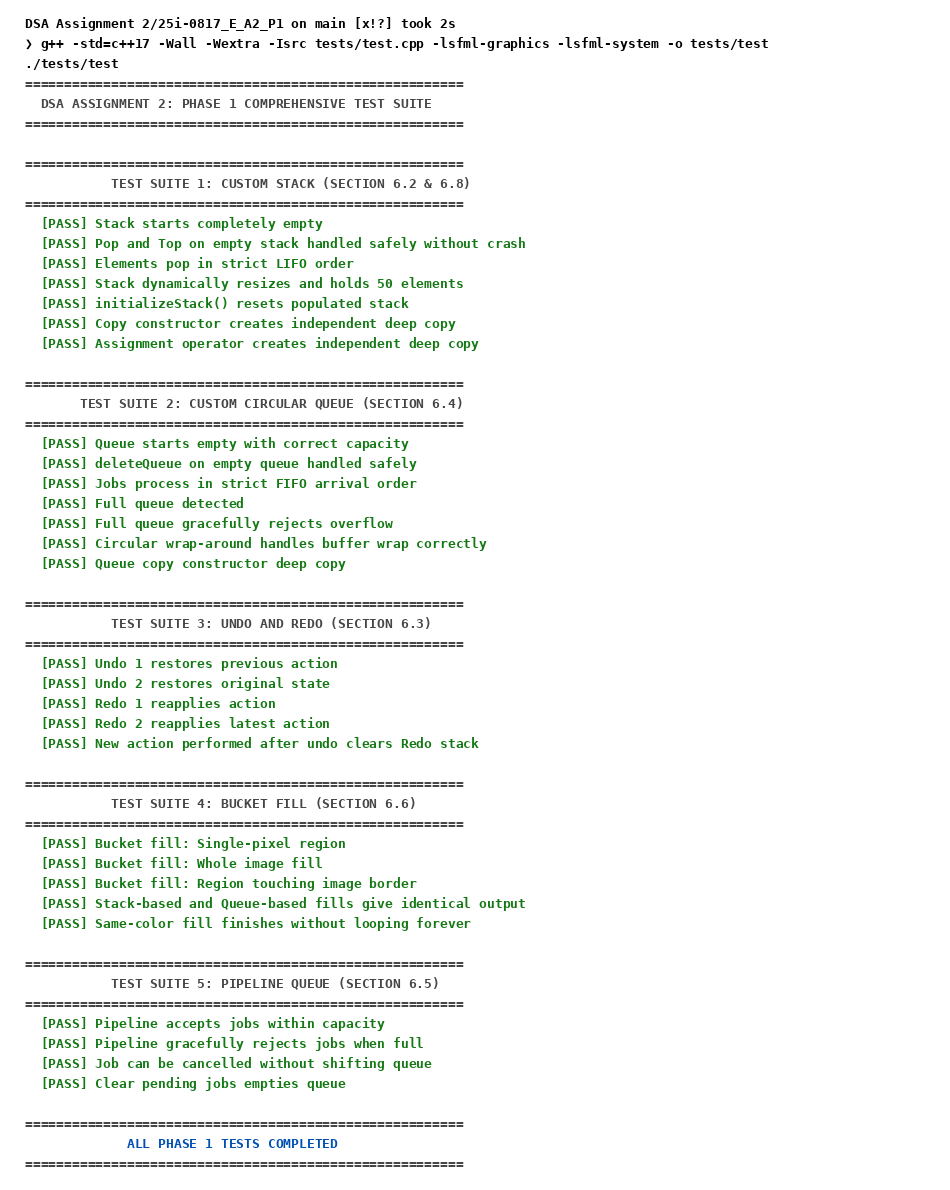
\includegraphics[width=0.74\textwidth,height=5.2cm,keepaspectratio]{test_results.png}
\end{center}

\end{document}
